\section{Multilayer Perceptron}

\subsection{Methods}
This section covers how we went about implementing the MLP back-progagation gradient descent algorithm and which parameters we chose to make it run optimally. 
\subsubsection{Treatment of Data}
First of all, we had to bring the data into a format where we could hand it over to our algorithm in a way that made training with early stopping possible.
\paragraph{Splitting}
The data was already available as separate training and test data. So, all what was left to do was to split the training data into a random $\frac{2}{3}$ training and $\frac{1}{3}$ validation set. This was easily achieved by computing a random permutation of the indices of the available data patterns and then dividing the dataset and the labelset at the $\frac{2}{3}$ mark according to the permutation.  
\paragraph{Preprocessing}
Preprocessing of the created training and validation as well as the test set was further achieved by computing the min. and max. features of the untouched training data beforehand and then applying the normalization as given the project instructions to the training and the test data. So, the actual preprocessing was done before splitting the data in order to keep the operation concise and not unnecessarily complicate it. 

\subsubsection{MLP setup}
The structure of the MLP we were advised to use through the project instructions is depicted in Fig. \ref{fig:mlp}. The differences to the two-layer MLP discussed in the lecture lie in the following properties: Firstly, the first hidden layer has double the outputs of a "normal" MLP perceptron. Secondly, the gating function $g(a_{2k+1}, a_{2k})$ takes pairs of values from the hidden layer accordingly and last but not least the last activation value is not passed through another gating function.
\begin{figure}[!h]
	\centering
	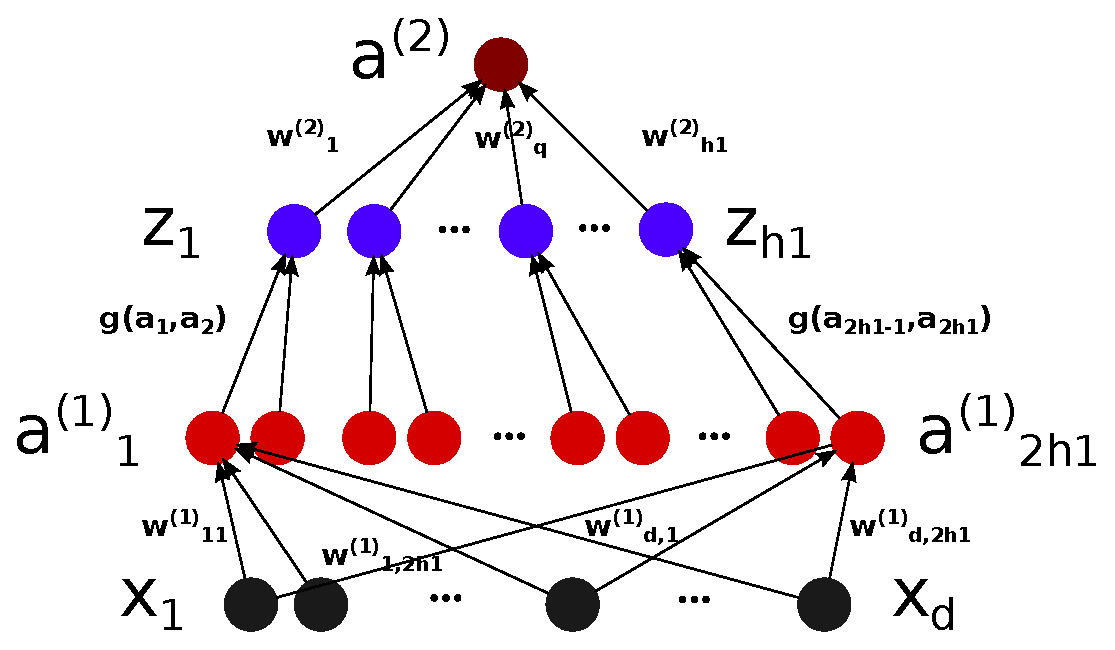
\includegraphics[width=.8\textwidth]{mlp/mlp.eps}
	\label{mlp}
	\caption{Schema of the MLP as described in the project instructions}
\end{figure}
\newline
\textsc{\textbf{TODO}}\\
Justify design and parameter choices\\
Show comparative plots illustrating the effects of learning rate, number of hidden units, momentum, etc. on\\
\begin{itemize}
\item overfitting
\item convergence speed
\end{itemize}
Comment on findings qualitatively

\paragraph{Early stopping}
Evaluate empirical error $\hat{R}(\hat{f};\mathcal{D}_V)$ for validation set $\mathcal{D}_V$ along-side the training-error $\hat{R}(\hat{f};\mathcal{D}_T)$while training the MLP on $\mathcal{D}_T$. Stop at the training at the epoch where the validation error stops decreasing and starts increasing. 
\subsubsection{Parameters for subtasks}

\subsubsection{Examples of overfitting}

\section{Results}